\documentclass[10pt,a4paper]{article}
\usepackage[paper=a4paper, hmargin=1.5cm, bottom=1.5cm, top=3.5cm]{geometry}

\usepackage[utf8]{inputenc}
\usepackage[spanish]{babel}

\usepackage{mathtools}
\usepackage{amsmath}
\usepackage{amsfonts}
\usepackage{amssymb}
\usepackage{listings}


\usepackage{booktabs}
\usepackage[table,xcdraw]{xcolor} % for setting colors
\usepackage{ifthen}
\usepackage{enumitem}
\usepackage{setspace}
\usepackage{wrapfig}

\usepackage{graphicx}
\usepackage{epstopdf}
\usepackage{tikz}
\usepackage[framemethod=tikz]{mdframed}
\usepackage{caption}
\usepackage{subcaption}
\usepackage{subfig}
\usepackage{float}

\usepackage{listings}
\usepackage[]{algorithm2e}

\DeclarePairedDelimiter{\ceil}{\lceil}{\rceil}

% set the default code style
\lstset{
    frame=tb, % draw a frame at the top and bottom of the code block
    tabsize=4, % tab space width
    showstringspaces=false, % don't mark spaces in strings
    %numbers=left, % display line numbers on the left
    commentstyle=\color{green}, % comment color
    keywordstyle=\color{blue}, % keyword color
    stringstyle=\color{red} % string color
}

\title{Organización del Computador II \\ TP3 \\ Tierra Pirata}

\newcommand{\order}[1]{$\mathcal{O}(#1)$}

\usetikzlibrary{calc}

\newcommand{\tikzmark}[1]{\tikz[overlay,remember picture] \node (#1) {};}
\newcommand{\DrawBox}[1][]{%
    \tikz[overlay,remember picture]{
    \draw[red,#1]
      ($(left)+(-0.2em,0.9em)$) rectangle
      ($(right)+(0.2em,-0.3em)$);}
}

%%%%%%%%%% Macros misceláneos - Inicio %%%%%%%%%%
\newcommand{\xmm}[1]{\texttt{XMM#1}\ }
\newcommand{\rax}{\texttt{RAX}\ }
\newcommand{\rbx}{\texttt{RBX}\ }
\newcommand{\rcx}{\texttt{RCX}\ }
\newcommand{\rdx}{\texttt{RDX}\ }
\newcommand{\rbp}{\texttt{RBP}\ }
\newcommand{\rsp}{\texttt{RSP}\ }
\newcommand{\mem}{\texttt{MEM}\ }
\newcommand{\reg}[1]{\texttt{#1}\ }
\newcommand{\asm}[1]{\texttt{\uppercase{#1}}\ }
\newcommand{\addr}[1]{\texttt{#1}\ }
\newcommand{\file}[1]{\texttt{#1}\ }
\newcommand{\command}[1]{\texttt{#1}\ }
\newcommand{\fun}[1]{\texttt{#1}\ }
\newcommand{\hex}[1]{\texttt{#1}\ }
%%%%%%%%%% Macros misceláneos - Fin %%%%%%%%%%

% Registros
\usepackage{array}
\newcolumntype{L}[1]{>{\raggedright\let\newline\\\arraybackslash\hspace{0pt}}m{#1}}
\newcolumntype{C}[1]{>{\centering\let\newline\\\arraybackslash\hspace{0pt}}m{#1}}
\newcolumntype{R}[1]{>{\raggedleft\let\newline\\\arraybackslash\hspace{0pt}}m{#1}}


\newcommand{\regfloats}[4]{\begin{tabular}{|C{2cm}|C{2cm}|C{2cm}|C{2cm}|}\hline
  #1 & #2 & #3 & #4 \\ \hline \end{tabular}}

\newcommand{\regintOcho}[8]{
  \vspace{0.3cm}
  \begin{tabular}{|C{1.3cm}|C{1.3cm}|C{1.3cm}|C{1.3cm}|C{1.3cm}|C{1.3cm}|C{1.3cm}|C{1.3cm}|}\hline
  #1 & #2 & #3 & #4 & #5 & #6 & #7 & #8  \\ \hline \end{tabular}
  \vspace{0.3cm}
}
\onehalfspacing
\begin{document}

%% cover page

\maketitle

\begin{figure}[H]
  \centering
    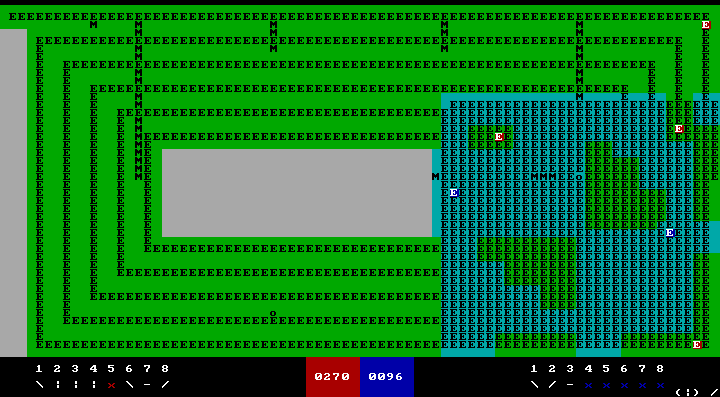
\includegraphics[scale=0.5]{images/game}
\end{figure}

\bigskip
\normalsize
\begin{table}[h]
\centering
\begin{tabular}{|l l l|}
\hline
Integrante       & \multicolumn{1}{c}{LU}     & Correo electrónico        \\ \hline
Christian Cuneo & \multicolumn{1}{c}{755/13} & chriscuneo93@gmail.com \\ 
Julián Bayardo & 850/13                      & julian@bayardo.com.ar \\
Martin Baigorria & 575/14          & martinbaigorria@gmail.com \\ \hline
\end{tabular}
\end{table}

\vfill

\begin{center}
\textbf{Reservado para la cátedra}
\end{center}
\begin{table}[h]
\centering
\begin{tabular}{|l|l|l|}
\hline
Instancia       & Docente & Nota \\ \hline
Primera entrega &         &      \\ \hline
Segunda entrega &         &      \\ \hline
\end{tabular}
\end{table}

\newpage
\tableofcontents

% end cover page

\pagebreak

\section{Introducción}

El objetivo del presente trabajo practico es aprender y aplicar diferentes conceptos de \textit{System Programming}. A partir de una implementación de un boot-sector, se programo un pequeño kernel con los diferentes mecanismos de protección y ejecución concurrente de tareas para luego poder ejecutar un juego con hasta 16 tareas concurrentes a nivel de usuario.

\subsection{Inicialización}

Al prender la computadora, comienza la inicializacion del \texttt{POST} (Power-On Self-Test), un programa de diagnostico de hardware que verifica que todos los dispositivos se han inicializado de manera correcta. Una vez terminado el \texttt{POST}, el \texttt{BIOS} se encarga de identificar el primer dispositivo de boooteo, ya sea un CD, un disco rígido o un diskette. En este trabajo, inicializaremos el sistema a partir de un diskette.

El \texttt{BIOS} (Basic Input-Output System) copia de memoria \texttt{RAM} los primeros 512 bytes del sector a partir de la direccion \addr{0x7c00} de un diskette. Esto se copia comenzando en la direccion \addr{0x1200} y luego se ejecuta el boot-sector a partir de allí. El boot-sector encuentra en el floppy el archivo \file{kernel.bin}, y luego lo copia en memoria a partir de la direccion \addr{0x1200}, ejecutando a partir de la misma.


\section{Kernel}

El \texttt{Kernel} es una parte esencial de los sistemas operativos modernos. Se ocupa de inicializar las diferentes estructuras necesarias para utilizar las diferentes funciones del procesador.

\section{Modo Real}

\subsection{Introducción}

Por una cuestión de compatibilidad hacia atrás, al inicializar un procesador Intel, el mismo funciona como un 8086, lo que conocemos como \texttt{Modo Real}. 

En \texttt{Modo Real}, no existe la protección por hardware, por lo que cualquier código en ejecución tiene acceso a todos los segmentos de memoria y puede utilizar cualquier instrucción del 8086. Para poder utilizar otras instrucciones y funcionalidades mas avanzadas y habilitar la protección por hardware, se debe pasar a Modo Protegido.

\subsection{A20}
El addressing line \texttt{A20} forma parte del bus de direcciones del procesador. En un \texttt{8086}, este bus tiene 20 lineas, numeradas de la 0 a la 19. Sin embargo, cuando salio al mercado el \texttt{80286}, el primero en soportar el modo protegido,  el bus de direcciones paso a tener 24 bits. El problema que surgió es que muchos programadores en su código del \texttt{8086} utilizaban lo que se conoce como wrap-around. Es decir, cuando accedían a memoria, utilizaban el overflow en el bus de direcciones como parte de la lógica de sus programas. El 80286 no soportaba este overflow, rompiendo la compatibilidad hacia atrás, dado que tenia 4 lineas de address adicionales.

Para solucionar este problema, a IBM se le ocurrió utilizar un pin del controlador del teclado que estaba sin usar y conectarlo a la linea 20 del bus de direcciones para poder forzar el overflow en los programas viejos. Por esta razón, antes de pasar a modo protegido se debe habilitar esta linea, para poder utilizar todo el espacio direccionable por todas las lineas del bus de direcciones.

\subsection{Global Descriptor Table}
Antes de poder pasar a modo protegido, debemos cargar la GDT. La GDT se encarga de asignar diferentes atributos de protección a los segmentos de memoria, para luego poder habilitar la protección por hardware. Esta estructura la armamos como un array de \texttt{gdt\_entry} en C.

\begin{figure}[h!]
  \centering
    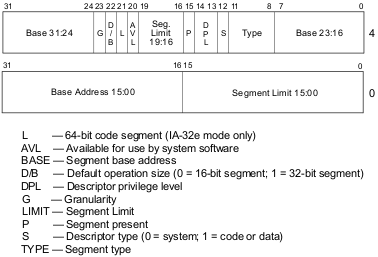
\includegraphics[width=0.5\textwidth]{images/segment_descriptor}
  \caption{Segment Descriptor}
\end{figure}

Luego, cargamos la GDT con el comando \command{lgdt} y el descriptor de la GDT armado desde C (\texttt{GDT\_DESC}).

\subsection{Pasaje a Modo Protegido}
Una vez armada la GDT y habilitado el A20, debemos habilitar Modo Protegido. El modo de protección esta definido por el bit menos significativo del registro \reg{CR0}. Usando un \& lógico, habilitamos este bit.

Una vez que tenemos todas las estructuras necesarias armadas, hay que hacer un \command{jump far} a alguno de los segmentos que definimos en la GDT. De esta forma finalmente habilitamos la protección por hardware y pasamos a Modo Protegido. 


\section{Modo Protegido}

\subsection{Selector de Segmento}
Al entrar a modo protegido, inicializamos los diferentes selectores de segmento. Los mismos tienen el siguiente formato:

\begin{figure}[h!]
  \centering
    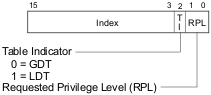
\includegraphics[scale=0.8]{images/segment_selector}
  \caption{Segment Selector}
\end{figure}

\subsection{Niveles de protección}

Intel soporta 4 niveles de protección diferentes, siendo 0 el mas alto y 4 el mas bajo. Por esa razón los bits de protección tienen 2 bits.

\begin{figure}[h!]
  \centering
    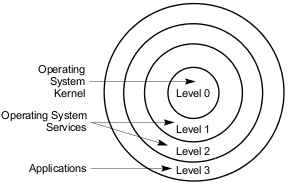
\includegraphics[width=0.4\textwidth]{images/protection_rings}
  \caption{IDT Descriptor}
\end{figure}

TODO: Escribir un poco como funciona la unidad de protección con RPL, DPL Y CPL.

\subsection{Interrupt Descriptor Table}

Una interrupción es una señal que le indica a la CPU que debe interrumpir la ejecución actual de instrucciones. El rol de la \texttt{IDT} (Interrupt Descriptor Table) es contener los diferentes descriptores de interrupcion y asociar las diferentes interrupciones a sus respectivas rutinas de atención de interrupción. Existen tres fuentes de interrupciones:

\begin{enumerate}
\item Hardware
\item Software
\item Internas
\end{enumerate}

A su vez, la \texttt{IDT} puede contener tres tipos de descriptores:

\begin{enumerate}
\item Interrupt Gate
\item Trap Gate
\item Task Gate
\end{enumerate}

Para construir la IDT, armamos primero en C la estructura \texttt{idt\_entry} con sus respectivos atributos y luego construimos un array de 256 posiciones del mismo (la máxima cantidad soportada por el procesador). En este trabajo practico solo utilizaremos descriptores de interrupción y de tarea.

\begin{figure}[h!]
  \centering
    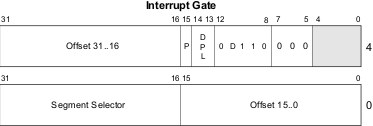
\includegraphics[width=0.5\textwidth]{images/idt_desc}
  \caption{IDT Descriptor}
\end{figure}

 Modificamos la macro de la cátedra para poder cargar la IDT con diferentes atributos. Luego inicializamos las diferentes posiciones que utilizamos con sus respectivos selectores de segmento y atributos, tomando también la referencia a las respectivas rutinas de atención.

Hay que tener mucho cuidado al settear los atributos. Caso contrario, al cambiar de segmento podemos tener un General Protection Fault (\#GP). Algunos atributos son:

\begin{enumerate}
\item P: Present flag. 1 if present.
\item DPL: Descriptor Protection Level. Nivel de privilegios del descriptor.
\item D: Size of gate. 1 = 32 bits; 0 = 16 bits.
\end{enumerate}

Un procesador Intel reserva por default las primeras 31 posiciones de la \texttt{IDT} para las diferentes excepciones del procesador. Actualmente, el procesador solo utiliza las primeras 21. Inicializamos estas excepciones del procesador a una rutina que imprime la excepción en pantalla.

Mas adelante inicializaremos otros descriptores de la \texttt{IDT} para atender otras interrupciones como la del reloj y la del teclado.

Una vez cargada la IDT, se debe remapear el PIC (Programmable Interrupt Controler) para referir a las nuevas interrupciones que agreguemos. Esto se hace con las rutinas de la catedra \texttt{resetear\_pic} y luego \texttt{habilitar\_pic}.

\subsection{Memory Management Unit}
Un procesador Intel, para gestionar lo que son los accesos a memoria, utiliza una \texttt{MMU} (Memory Management Unit). La misma esta compuesta por la Unidad de Segmentación y la Unidad de Paginación.

\begin{figure}[H]
  \centering
    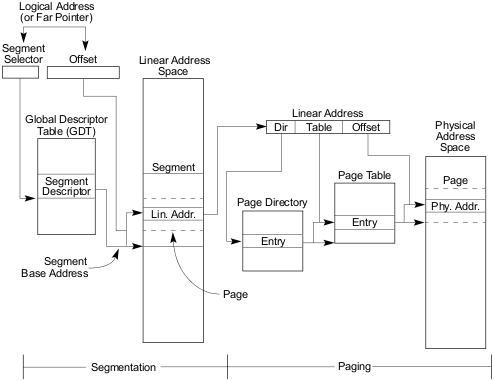
\includegraphics[width=0.6\textwidth]{images/memory_management}
  \caption{Segmentation \& Paging}
\end{figure}

La paginacion nos permite que cada tarea pueda tener su propia \texttt{memoria virtual}, mappeando direcciones físicas a direcciones virtuales.

\subsubsection{Unidad de Segmentación}

La unidad de segmentación se ocupa de pasar desde las \textit{direcciones lógicas} a direcciones lineales. Para ello, utiliza la GDT para identificar el segmento adecuado y luego su respectivo offset. La unidad de protección verifica que el \texttt{RPL} es compatible con el \texttt{CPL} y el \texttt{DPL}.

En modo protegido, los selectores de segmento tienen 16 bits. Los 13 bits mas significativos contienen el indice dentro de la tabla de descriptores. El bit 2 especifica si la operación utiliza la \texttt{GDT} o la \texttt{LDT}. Finalmente, los 2 bits menos significativos definen el nivel de privilegio solicitado.

\subsubsection{Unidad de Paginación}

Para activar la paginación, en primer lugar debemos inicializar el directorio de paginas y cargar el registro \reg{cr3} con la dirección del mismo. Como los directorios de paginas estan alineados a 4 kb, los primeros 20 bits del cr3 no son necesarios para identificar el directorio, por lo que son utilizados por atributos del procesador. En nuestro caso no utilizamos estos atributos, por lo que son todos 0.

Luego, debemos activar la paginacion con el ultimo bit del registro \reg{cr0}.

Si la paginación esta activada, la dirección lineal luego pasa por la unidad de paginación. La unidad de paginación se encarga de ir desde la dirección lineal a la dirección física en memoria. En caso de que la dirección lineal no este paginada, el procesador tiene una page fault exception.

Para facilitar el manejo del armado de estructuras para la paginación, se crearon las siguientes funciones en C. Antes de explicar que hace cada función, un comentario. Cada directorio de paginas tiene 1024 entradas de descriptores de 4 bytes. Lo mismo sucede con los directorios de paginas, que también tienen 1024 entradas con descriptores de 4 bytes. El procesador, al buscar estas estructuras en memoria RAM, requiere que las mismas estén alineadas a 4kb, dado que es el tamaño de pagina que carga en memoria cache.

\begin{enumerate}
\item \fun{create\_page\_table(uint directoryBase, uint directoryEntry, uint physicalAddress, uchar readWrite, uchar userSupervisor)}: Asigna una \texttt{page\_table} a una tabla de directorios con los atributos pasados por parametro. Al final de la función, se limpia la memoria cache para garantizar que cuando el procesador busca esta pagina, la misma se encuentra actualizada.

\item \fun{delete\_page\_table(uint directoryBase, uint directoryEntry)}: Borra una tabla de paginas de un directorio de paginas. Esto lo hace simplemente setteando el bit P (present) en cada pagina en 0.

\item \fun{create\_page(uint directoryBase, uint directoryEntry, uint tableEntry, uint physicalAddress, \\ uchar readWrite, uchar userSupervisor)}: Crea una pagina en la tabla de paginas de algún directorio.

\item \fun{delete\_page(uint directoryBase, uint directoryEntry, uint tableEntry)}: Borra una pagina en la tabla de paginas de algún directorio. Esto lo hace setteando el bit P en 0.

\item \fun{mmap(uint virtualAddress, uint physicalAddress, uint directoryBase, uchar readWrite, \\ uchar userSupervisor)}: Mappea una dirección virtual en una direccion fisica. Para esto, primero se busca la tabla de paginas y la pagina correspondiente a la dirección virtual. Luego se le asigna a esa pagina la dirección física. Esto se hace de la siguiente forma:
	\begin{enumerate}
	\item A partir de la dirección virtual, se busca la entrada de directorio correspondiente a la misma. Esto se hace dividiendo el virtualAdress por el tamaño direccionable por cada page\_directory.$virtualAdress / 1024*4kb$. Esto es equivalente a $virtualAdress >> 22$.
	\item Buscamos el indice en la entrada de paginas. Esto se calcula dividiendo por el tamaño de pagina e ignorando los bits correspondientes a la entrada de directorio $virtualAdress / 4kb$ $\&$ $0x3FF$, que es equivalente a $virtualAdress >> 12$ $\&$ $0x3FF$.
	\end{enumerate}

\item \fun{munmap(uint directoryBase, uint virtualAddress)}: Desmappea la pagina correspondiente a una dirección virtual. Calcula todos los indices necesarios de la misma manera que \fun{mmap}

\item \fun{mmu\_inicializar\_dir\_kernel()}: Inicializa el directorio del kernel. Para ello, hacemos memory mapping sobre el kernel y le asignamos un area libre, todo desde \addr{0x00000000} a \addr{0x003FFFF}.

\item \fun{mmu\_inicializar\_dir\_pirata(uint directoryBase, uint pirateCodeBaseSrc, uint pirateCodeBaseDst)}: Esta función inicializa el directorio de un pirata. Al igual que el Kernel, hacemos memory mapping, aunque en modo user y en read only. A su vez, mappeamos la pagina donde vamos a poner el codigo del pirata, y copiamos el código del pirata que se encuentra en el Kernel en esta pagina.

\item \fun{mmu\_move\_codepage(uint src, uint dst, pirata\_t *p)}: Mueve la pagina de codigo del pirata desde $src$ a $dst$.

No implementamos la funcion \texttt{mmu\_inicializar} dado que todo el trabajo lo hace \texttt{mmu\_inicializar\_dir\_kernel}.

\end{enumerate}

\subsection{Otras Interrupciones}

Para inicializar otras interrupciones, tenemos que agregar los diferentes descriptores a la IDT, que apuntan a su correspondiente rutina de atención y ademas tienen los atributos correctos. Recordemos que las rutinas de atención de la interrupción deben ser transparentes a lo que el procesador estaba ejecutando en el momento, por lo que se debe guardar todos los registros y luego restaurarlos al finalizar la rutina de atención. Ademas, las interrupciones en general llevan a un escalamiento de privilegios, por lo que los privilegios también deben ser restaurados.

A su vez, la rutina de atención de la interrupción debe indicarle al pic que la interrupción esta siendo atendida, para que otras interrupciones puedan suceder. Esto se hace con la función de la cátedra \fun{fin\_intr\_pic1}.

\subsubsection{Reloj}

Esta es una interrupción interna, que sucede con cada \texttt{tick} del reloj del procesador. La rutina de atención de esta interrupción se encarga de mostrar la animación de un cursor rotando en la esquina inferior derecha de la pantalla, por medio de la función \fun{screen\_actualizar\_reloj\_global}.

\subsubsection{Teclado}
Utilizaremos la rutina de atención del teclado para habilitar las diferentes teclas disponibles a los jugadores. Cuando programábamos esto, notamos que es necesario tomar la tecla presionada desde el controlador del teclado, caso contrario el teclado no vuelve a solicitar una interrupción.

\subsubsection{Software}
Asignamos a la interrupción \addr{0x46} (70) una rutina que atiende un servicio del sistema.

\subsection{Task State Segment}

La \texttt{TSS} (Task State Segment) es el espacio de memoria previsto en los procesadores \texttt{IA-32} como el espacio de contexto de cada tarea. Este segmento debe tener su respectivo descriptor en la \texttt{GDT}. Ademas, el selector de segmento de la tarea que se
esta ejecutando actualmente se debe encontrar en el registro \reg{TR} (Task Register).

Para llamar a una tarea, se lleva a cabo un \texttt{call far} con su respectivo selector de segmento. Si ya estabamos ejecutando una tarea, se guarda su contexto en \reg{TR} antes de ejecutar la nueva tarea. 

La primera vez que llamamos a una tarea, el registro \reg{TR} no tiene un valor definido. Ademas, debemos guardar el contexto del programa en ejecucion. Para ello, se crea una tarea inicial  en la \texttt{TSS} para que el procesador tenga donde guardar el contexto actual.

\begin{figure}[H]
  \centering
    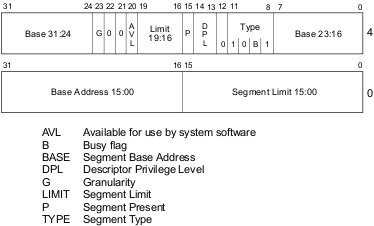
\includegraphics[width=0.6\textwidth]{images/tss_descriptor}
  \caption{TSS Descriptor}
\end{figure}

\begin{figure}[H]
  \centering
    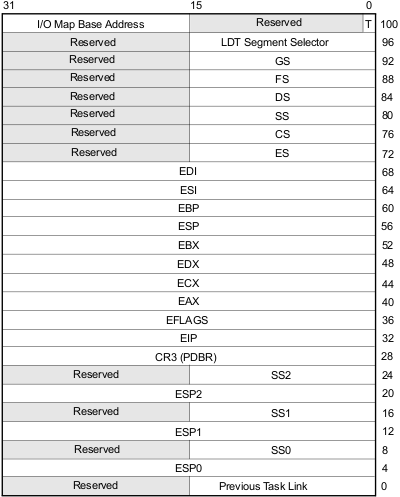
\includegraphics[width=0.6\textwidth]{images/tss}
  \caption{Task State Segment}
\end{figure}

\begin{figure}[H]
  \centering
    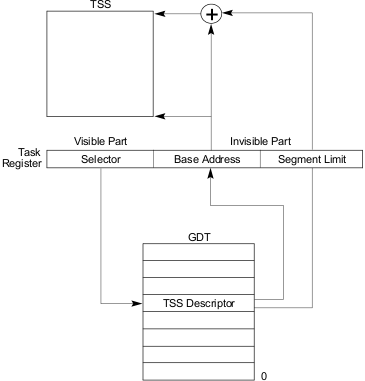
\includegraphics[width=0.6\textwidth]{images/task_register}
  \caption{Segmentation \& Paging}
\end{figure}

\subsection{Scheduler}
\section{Tierra Pirata}

\subsection{Memory Management Functions}
Para facilitar el manejo del armado de estructuras para la paginación, se crearon las siguientes funciones en C. Antes de explicar que hace cada función, un comentario. Cada directorio de paginas tiene 1024 entradas de descriptores de 4 bytes. Lo mismo sucede con los directorios de paginas, que también tienen 1024 entradas con descriptores de 4 bytes. El procesador, al buscar estas estructuras en memoria RAM, requiere que las mismas estén alineadas a 4kb, dado que es el tamaño de pagina que carga en memoria cache.

\begin{enumerate}
\item \fun{create\_page\_table(uint directoryBase, uint directoryEntry, uint physicalAddress, uchar readWrite, uchar userSupervisor)}: Asigna una \texttt{page\_table} a una tabla de directorios con los atributos pasados por parametro. Al final de la función, se limpia la memoria cache para garantizar que cuando el procesador busca esta pagina, la misma se encuentra actualizada.

\item \fun{delete\_page\_table(uint directoryBase, uint directoryEntry)}: Borra una tabla de paginas de un directorio de paginas. Esto lo hace simplemente setteando el bit P (present) en cada pagina en 0.

\item \fun{create\_page(uint directoryBase, uint directoryEntry, uint tableEntry, uint physicalAddress, \\ uchar readWrite, uchar userSupervisor)}: Crea una pagina en la tabla de paginas de algún directorio.

\item \fun{delete\_page(uint directoryBase, uint directoryEntry, uint tableEntry)}: Borra una pagina en la tabla de paginas de algún directorio. Esto lo hace setteando el bit P en 0.

\item \fun{mmap(uint virtualAddress, uint physicalAddress, uint directoryBase, uchar readWrite, \\ uchar userSupervisor)}: Mappea una dirección virtual en una direccion fisica. Para esto, primero se busca la tabla de paginas y la pagina correspondiente a la dirección virtual. Luego se le asigna a esa pagina la dirección física. Esto se hace de la siguiente forma:
	\begin{enumerate}
	\item A partir de la dirección virtual, se busca la entrada de directorio correspondiente a la misma. Esto se hace dividiendo el virtualAdress por el tamaño direccionable por cada page\_directory.$virtualAdress / 1024*4kb$. Esto es equivalente a $virtualAdress >> 22$.
	\item Buscamos el indice en la entrada de paginas. Esto se calcula dividiendo por el tamaño de pagina e ignorando los bits correspondientes a la entrada de directorio $virtualAdress / 4kb$ $\&$ $0x3FF$, que es equivalente a $virtualAdress >> 12$ $\&$ $0x3FF$.
	\end{enumerate}

\item \fun{munmap(uint directoryBase, uint virtualAddress)}: Desmappea la pagina correspondiente a una dirección virtual. Calcula todos los indices necesarios de la misma manera que \fun{mmap}

\item \fun{remap(uint directoryBase, uint virtualAddress, uint physicalAddress)}: Remappea la pagina dada por el $virtualAddress$ a la dirección $physicalAddress$.

\item \fun{getPhysVirt(uint directoryBase, uint virtualAddress)}: A partir de un $virtualAddress$, devuelve el $physicalAddress$.

\item \fun{isMapped(uint directoryBase, uint virtualAddress)}: Devuelve si la dirección virtual esta mappeada en memoria.

\item \fun{mmu\_inicializar\_dir\_kernel()}: Inicializa el directorio del kernel. Para ello, hacemos memory mapping sobre el kernel y le asignamos un area libre, todo desde \addr{0x00000000} a \addr{0x003FFFF}.

\item \fun{mmu\_inicializar\_dir\_pirata(uint directoryBase, uint pirateCodeBaseSrc, uint pirateCodeBaseDst)}: Esta función inicializa el directorio de un pirata. Al igual que el Kernel, hacemos memory mapping, aunque en modo user y en read only. A su vez, mappeamos la pagina donde vamos a poner el codigo del pirata, y copiamos el código del pirata que se encuentra en el Kernel en esta pagina.

\item \fun{mmu\_move\_codepage(uint src, uint dst, pirata\_t *p)}: Mueve la pagina de codigo del pirata desde $src$ a $dst$.

No implementamos la funcion \texttt{mmu\_inicializar} dado que todo el trabajo lo hace \texttt{mmu\_inicializar\_dir\_kernel}.

\end{enumerate}

\subsection{Interrupciones}

\subsubsection{Reloj}

La interrupción de reloj comienza llamando la función \fun{scheduler\_tick}, que se ocupa de devolver el indice de la tarea en la \texttt{GDT} al que se debe ir. En caso de que se tenga que intercambiar de tarea, la rutina de atención de esta interrupción hace un \texttt{jump far} a la nueva tarea.

\subsubsection{Teclado}

Cuando hay una interrupción de teclado, la tecla que ha sido presionada se codifica con un \texttt{scan code} de 8 bits, que se guarda en el controlador de teclado. Estas se leen a través del puerto \hex{0x60} con la instrucción \texttt{in al, 0x60}. Una vez guardado el código, se llama a la función de C \fun{isr\_keyboard}, a la que se le pasa el código por pila respetando la convención C de 32 bits.

La función \fun{isr\_keyboard} luego le asigna diferentes funciones a las teclas \texttt{right\_shift}, \texttt{left\_shift} e \texttt{y}. Todos los scan codes están definidos en \texttt{keyboardcodes.h}.

\subsubsection{Syscall}
El sistema provee un servicio a las diferentes tareas mediante la interrupción \hex{0x46}. La misma le permite a las tareas usar de forma indirecta las siguientes funciones.
\begin{enumerate}
\item \fun{game\_syscall\_pirata\_mover}: Mueve al pirata de una posición a otra. Si el pirata que llamo a esta función es un minero, requiere que la pagina a la que  se quiere mover ya este paginada. Al moverse el pirata, también se mueve su código, y se debe también remappear la dirección \addr{0x400000} a la nueva dirección física donde el código se ha movido.

Si un pirata explorador al moverse encuentra un tesoro, se lanza un pirata minero automáticamente. Al mismo se le debe pasar la posición del tesoro por parámetro. Utilizando la convención C y el stack correspondiente a la nueva tarea, escribimos los parámetros en el stack de la dirección física de su respectivo codigo.

Cuando programamos esto tuvimos el siguiente problema. La interrupcion al mover causaba un escalamiento de privilegios, pero seguiamos manteniendo el \reg{cr3} de la tarea que encontró el tesoro. Por esta razon no podiamos escribir en el stack de la nueva tarea y teniamos un \#GP Fault. Esto se debe a que las tareas tienen paginadas la memoria en solo lectura. Para resolver esto, simplemente cambiamos el \reg{cr3} por el del kernel antes de escribir en el stack y luego lo restauramos.

\item \fun{game\_syscall\_cavar}: Actualiza los puntajes y los atributos del tesoro correspondiente cuando un pirata minero cava. En caso de que se acaben las monedas del tesoro, el pirata se desaloja con la función \fun{game\_pirata\_exploto}
\item \fun{game\_syscall\_pirata\_posicion}: Devuelve la posición del pirata. La misma se codifica como y $<<$ 8 $|$ x en un entero.
\end{enumerate}

El Syscall se llama indirectamente a través de \texttt{inline asm}, que se ocupa de pasar los parámetros y llamar a la respectiva función. Al ejecutar esta interrupción hay un escalamiento de privilegios a nivel 0, lo que permite manipular la memoria y ejecutar funciones que no se podrían ejecutar desde una tarea (user), como por ejemplo manipular los directorios de pagina.

\pagebreak

\subsection{Scheduler}

El Scheduler es una función en C que es llamada por la interrupción de teclado. La misma de identificar la tarea que se debe ejecutar actualmente para respetar el siguiente diagrama:

\begin{figure}[H]
  \centering
    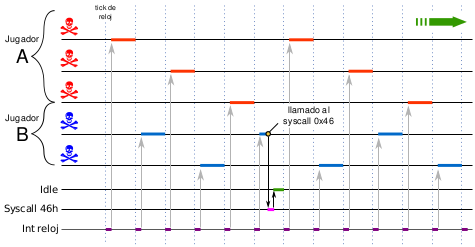
\includegraphics[width=0.7\textwidth]{images/scheduler}
  \caption{Diagrama de Tareas}
\end{figure}

Mantiene un contador para saber por cuantos ciclos de clock se ha ejecutado la tarea actual. A su vez, mantiene un flag para identificar a que jugador pertenece la ultima tarea que ha sido ejecutada. Para identificar que tarea ejecutar, itera sobre los piratas del jugador a partir del actual. Una tarea es ejecutada a lo sumo \texttt{SCHEDULER\_TASK\_TICKS} ciclos de clock. Esto esta definido en \texttt{defines.h}.

El intercambio con la tarea \texttt{Idle} cuando sucede un \texttt{Syscall} o cuando se desaloja a un pirata lo maneja la rutina de assembler en \texttt{isr.asm}. El Scheduler simplemente reemplaza la tarea actual por la próxima a ejecutar.

\subsection{Estructuras}

Para mantener cuenta del estado del juego y de cada uno de los jugadores, creamos algunas estructuras definidas en \texttt{game.h}. Para saber que posiciones del mapa ya han sido paginadas, cada jugador mantiene un \texttt{bit\_map} con (\texttt{MAPA\_ALTO} * \texttt{MAPA\_ANCHO} / 8) chars. Cada bit corresponde a una pagina del mapa. De esta manera, al mover un jugador podemos fácilmente identificar que paginas deben ser mappeadas.

%\pagebreak


%\subsection{Funciones Auxiliares}
%Para facilitar la programación del juego, utilizamos las siguientes funciones auxiliares:

%\begin{enumerate}
%\item \fun{void game\_pirata\_erigir(pirata\_t *pirata, jugador\_t *j, uint tipo)}: 
%\item \fun{void game\_pirata\_habilitar\_posicion(jugador\_t *j, pirata\_t *pirata, int x, int y)}: 
%\item \fun{void game\_pirata\_exploto(uint id)}: 
%\item \fun{void game\_jugador\_setBitMapPos(jugador\_t *j, uint x, uint y, uchar val)}: 
%\item \fun{char game\_jugador\_getBitMapPos(jugador\_t *j, uint x, uint y)}: 
%\item \fun{void game\_pirata\_paginarPosMapa (pirata\_t *p, int x, int y)}: 
%\item \fun{void game\_jugador\_paginarPosMapa\_piratasExistentes (jugador\_t *j, int x, int y)}: 
%\item \fun{uint game\_xy2addressPhys(int x, int y)}: 
%\item \fun{uint game\_xy2addressVirt(int x, int y)}: 
%\item \fun{uint game\_posicion\_valida(int x, int y)}: 
%\item \fun{int game\_jugador\_taskAdress(jugador\_t *j, pirata\_t *p)}: 
%\item \fun{void game\_updateScreen(pirata\_t * p, jugador\_t * j, int x, int y)}: 
%\item \fun{uint game\_pirateIdtoDirectoryAddress(uint id)}: 
%\item \fun{pirata\_t* id\_pirata2pirata(uint pirate\_id)}: 
%\item \fun{uint game\_dir2xy(direccion dir, int *x, int *y)}: 
%\end{enumerate}

\subsection{Tareas}

\subsubsection{Idle}
La tarea Idle simplemente tiene un contador que sirve  para actualizar el reloj del juego.

\subsubsection{Explorador y Minero}
Estas tareas simplemente usan los syscalls para moverse por el mapa. No tocamos el código original de la cátedra. Utilizamos el código del minero del jugador A en el minero del jugador B.

\end{document}

